\documentclass{amsart}

%packeges used in this document
\usepackage{amsrefs}
\usepackage{comment}
\usepackage{graphicx}
\usepackage{subcaption}
\usepackage[section]{placeins}

\title
[Examination of the Cross Product] % shortened title for headings
{Examination of the Cross Product as a Special Case of the Exterior Product in Three Dimensions}

\author{William Clampitt}
\date{November 24, 2017}

\keywords{Exterior Product, Cross Product, Vector, Bivector, Multivector, Psudovector}



\begin{document}	
	\begin{abstract}
		In Calculus III students are introduced to the cross product of two vectors in three-dimensional, Euclidean space. The cross-product exhibits properties, such as being normal tp the original two vectors and having a magnitude equal to that of the area formed by the original two vectors. In exterior algebra, this operation is described by the exterior product. The exterior product creates a multi-vector that describes the parallelogram formed by the original two vectors with a clockwise or counter clockwise orientation. Through this research, properties of the cross product are explained in terms of the exterior product to clarify the seemingly random properties displayed by the cross product. My research into these relationships was conducted by researching other scholarly articles about the exterior product and its properties and comparing them to those exhibited by the cross product. The results of this comparison show a possibly more intuitive way of looking at relationships between two vectors in space.
	\end{abstract}

	\maketitle
	\newpage
	
%%%%%%%%%%%%%%%%%%%%%%%%%%%%%%%%%%%%%%%%%%%%%%%%%%%%%%%%%%%%%%%%%%%%%%%%%%%%%%%%%%%%%%%%%%%%%%%%%%%%%%%%%%%%%%%%%%%%%%%%%%%%%%%%%%%%%%%%%%%%%%%%%%%%%%%%%%%%%%%%%%%%%%%%%%%%%%%%%%%%%%%%%%%%%%%%%%%%%%%%%%%%%%%%%%%%%%%%%%%%%%%%%%%%%%%%%%%%%%%%%%%%%%%%%%%%%%%%%%%%%%%%%%%%%%%%%%%%%%%%%%%%%%%%%%%%%%%%%%%%%%%%%%%%%%%%%%%%%%%%%%%%%%%%%%%%%%%%%%%%%%%%%%%%%%%%%%%%%%%%%%%%%%%%%%%%%%%%%%%%%%%%%%%%%%%%%%%%%%%%%%%%%%%%%%%%%%%%%%%%%%%%%%%%%%%%%%%%		
	\section{Introduction} \label{intro}
		In Calculus III, students are, often for the first time, introduced to the cross product. The cross product takes two vectors in three dimensions and creates a normal vector with a magnitude equal to that of the area formed by the original two vectors. In reality, what the students are actually doing is taking the exterior product of a vector in three dimensions and are creating a three dimensional bi-vector that represents the parallelogram formed by  the two vectors. The reality of what the cross product is originates from a branch of mathematics called Exterior Algebra, which is far above the level of mathematics that the students are currently working in when they first learn about the cross product. The simplification of the exterior product as the cross product for three dimensions is needed for necessity for students to benefit from the usefulness of the exterior product, even though they are not at a level of math to fully understand what is happening. This simplification of generalized concepts for a specific use case happens very frequently in the study of mathematics in order to prevent students from being overwhelmed by a mass of abstract concepts by giving students incremental knowledge and then expanding on it in the future as they progress. Through this paper, a closer look will be taken at properties of the exterior product and how they translate to the properties students learn about the cross product.
		
%%%%%%%%%%%%%%%%%%%%%%%%%%%%%%%%%%%%%%%%%%%%%%%%%%%%%%%%%%%%%%%%%%%%%%%%%%%%%%%%%%%%%%%%%%%%%%%%%%%%%%%%%%%%%%%%%%%%%%%%%%%%%%%%%%%%%%%%%%%%%%%%%%%%%%%%%%%%%%%%%%%%%%%%%%%%%%%%%%%%%%%%%%%%%%%%%%%%%%%%%%%%%%%%%%%%%%%%%%%%%%%%%%%%%%%%%%%%%%%%%%%%%%%%%%%%%%%%%%%%%%%%%%%%%%%%%%%%%%%%%%%%%%%%%%%%%%%%%%%%%%%%%%%%%%%%%%%%%%%%%%%%%%%%%%%%%%%%%%%%%%%%%%%%%%%%%%%%%%%%%%%%%%%%%%%%%%%%%%%%%%%%%%%%%%%%%%%%%%%%%%%%%%%%%%%%%%%%%%%%%%%%%%%%%%%%%%%%		
	\section{Current Use of the Cross Product} \label{cross}
		The vector cross product as taught in Calculus III is an operation that takes two vectors in $\mathbb{R}^3$, and creates a vector, also in $\mathbb{R}^3$ that is normal to the original two vectors and has a magnitude equal to the area of the parallelogram formed by the two original vectors. The cross product has many applications in Calculus III, such as finding the curl of a vector, tangent planes to curves, torque, and finding the surface area of a function. The cross product is found by taking the determinant of the matrix (Equation~\ref{cross}). 
		
		\begin{gather}
			\label{cross}
				\mathbf{a} \times \mathbf{b} = 
					\begin{vmatrix} 
					\mathbf{e_1}&\mathbf{e_2}&\mathbf{e_3}\\
					a_1&a_2&a_3\\
					b_1&b_2&b_3
					\end{vmatrix}\\  
			\nonumber \\
			\nonumber
			\mathbf{a} \times \mathbf{b} = (a_2 b_3 - a_3 b_2)\mathbf{e_1} + (a_3 b_1 - a_1 b_3)\mathbf{e_2} + (a_1 b_2 - a_2 b_1)\mathbf{e_3}
		\end{gather}\\

		
		(Note: $\mathbf{e_1}$, $\mathbf{e_2}$, and $\mathbf{e_3}$ are the standard basis vectors for $\mathbb{R}^3$) As seen in Figure ~\ref{crosspic}, the cross product between these two vectors creates another vector that is orthogonal to $\mathbf{a}$ and $\mathbf{b}$.
		

		\begin{comment}
			Be sure to come back and insert pictures
		\end{comment}
		
		\begin{figure}
			\centering
			\begin{subfigure}{.45\linewidth}
				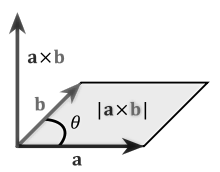
\includegraphics[width=\linewidth]{Fall_2017_Math_Research_Paper_Visuals/Cross_Product_Internet}
				\caption{$\mathbf{a} \times \mathbf{b}$}
				\label{crosspic}
			\end{subfigure}
			\begin{subfigure}{.45\linewidth}
				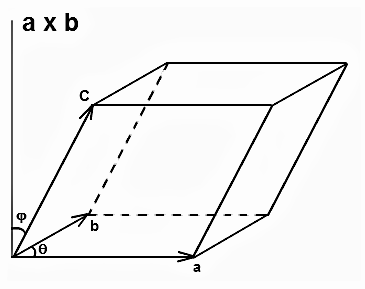
\includegraphics[width=.9\linewidth]{Fall_2017_Math_Research_Paper_Visuals/Triple_Scalar_Product_Internet_Visual}
				\caption{$(\mathbf{a} \times \mathbf{b}) \bullet \mathbf{c}$}
				\label{triplescalarproduct}
			\end{subfigure}
			\caption{}
			\label{cross}
		\end{figure}
				
	As stated above, this vector that is created is extremely useful for many applications, such as finding planes containing two vectors, tangent planes, the curl of a vector function, and surface area of functions.
	
%%%%%%%%%%%%%%%%%%%%%%%%%%%%%%%%%%%%%%%%%%%%%%%%%%%%%%%%%%%%%%%%%%%%%%%%%%%%%%%%%%%%%%%%%%%%%%%%%%%%%%%%%%%%%%%%%%%%%%%%%%%%%%%%%%%%%%%%%%%%%%%%%%%%%%%%%%%%%%%%%%%%%%%%%%%%%%%%%%%%%%%%%%%%%%%%%%%%%%%%%%%%%%%%%%%%%%%%%%%%%%%%%%%%%%%%%%%%%%%%%%%%%%%%%%%%%%%%%%%%%%%%%%%%%%%%%%%%%%%%%%%%%%%%%%%%%%%%%%%%%%%%%%%%%%%%%%%%%%%%%%%%%%%%%%%%%%%%%%%%%%%%%%%%%%%%%%%%%%%%%%%%%%%%%%%%%%%%%%%%%%%%%%%%%%%%%%%%%%%%%%%%%%%%%%%%%%%%%%%%%%%%%%%%%%%%%%%%		
	
	\section{The Exterior Product} \label{ext}
		The exterior product, often referred to as the wedge product because of its wedge shaped symbol $\wedge$, is a product defined in all dimensions that takes graded elements of the same dimension and creates a higher grade element. Graded elements refer to whether an element is a scalar, vector, bi-vector, etc. (Table ~\ref{tb:1}).
		
		% Table showing grade values of multivectors
		\begin{table}[h]
			\caption{Grade Assignment}
			\label{tb:1}
			\begin{tabular}{c | c}
				Element & Grade\\
				scalar & 0\\
				vector & 1\\
				bi-vector & 2\\
				tri-vector & 3\\
				n-vector & n
			\end{tabular}
		\end{table}
	
		These graded elements represent different types of oriented objects, but this paper focuses primarily on bi-vectors and tri-vectors. To show how a bi-vector is obtained via the exterior product, an example of the exterior product, between two three dimensional vectors is worked out in Equation ~\ref{bi}.\\

		\begin{gather*}
				\mathbf{a} = a_1 \mathbf{e_1} + a_2 \mathbf{e_2} + a_3 \mathbf{e_3} \nonumber\\
				\mathbf{b} = b_1 \mathbf{e_1} + b_2 \mathbf{e_2} + b_3 \mathbf{e_3} \nonumber\\
		\end{gather*}
	
		\begin{gather}
			\label{bi}
			\mathbf{a} \wedge \mathbf{b} = (a_1 \mathbf{e_1} + a_2 \mathbf{e_2} + a_3 \mathbf{e_3}) \wedge (b_1 \mathbf{e_1} + b_2 \mathbf{e_2} + b_3 \mathbf{e_3}) \\
			\downarrow \nonumber \\
			\mathbf{a} \wedge \mathbf{b} = (a_2 b_3 - a_3 b_2)(\mathbf{e_2} \wedge \mathbf{e_3}) + (a_3 b_1 - a_1 b_3)(\mathbf{e_3} \wedge \mathbf{e_1}) + (a_1 b_2 - a_2 b_1)(\mathbf{e_1} \wedge \mathbf{e_2})
			\nonumber
		\end{gather} \\
		
		When comparing this bi-vector to the vector that was obtained by taking the cross product between $\mathbf{a}$ and $\mathbf{b}$ in Section ~\ref{cross}, the coefficients are identical. The only difference is that with the exterior product, the operation creates a grade 2 element, or a bi-vector. Because the number of basis elements of the result equals the number of basis elements in the original two vectors, mathematicians refer to this output as a "pseudovector."

%%%%%%%%%%%%%%%%%%%%%%%%%%%%%%%%%%%%%%%%%%%%%%%%%%%%%%%%%%%%%%%%%%%%%%%%%%%%%%%%%%%%%%%%%%%%%%%%%%%%%%%%%%%%%%%%%%%%%%%%%%%%%%%%%%%%%%%%%%%%%%%%%%%%%%%%%%%%%%%%%%%%%%%%%%%%%%%%%%%%%%%%%%%%%%%%%%%%%%%%%%%%%%%%%%%%%%%%%%	
		\subsection{What are bi-vectors?}\label{sub:3.1} 
			Vectors are usually described as having a magnitude and a direction, but a bi-vector can be thought of as having two directions and a magnitude, hence the prefix  "bi". A bi-vector represents an oriented plane segment, much like how a vector is thought of as an oriented line segment. The two directions of a bi-vector come from the two vectors that came together to form the bi-vector and the magnitude is equivalent to the area of the parallelogram encompassed by those original vectors.
			
			The orientation of a bi-vector is described by either being clockwise or counter-clockwise. Since mathematicians traditionally operate in a right-handed coordinate system, if a bi-vector has a counter-clockwise orientation it is said to be positive (Figure ~\ref{bivectorpositive}), and if it has a clockwise orientation, it is said to be negative (Figure ~\ref{bivectornegative}).
			
			\begin{figure}[h]
				\centering
				\begin{subfigure}{0.45\linewidth}
					\includegraphics[width=\linewidth]{Fall_2017_Math_Research_Paper_Visuals/bivector_positive.png}
					\caption{Positive Orientation}
					\label{bivectorpositive}
				\end{subfigure}
				\begin{subfigure}{0.45\linewidth}
					\includegraphics[width=\linewidth]{Fall_2017_Math_Research_Paper_Visuals/bivector_negative.png}
					\caption{Negative Orientation}
					\label{bivectornegative}
				\end{subfigure}	
				\caption{}
				\label{bivectors}
			\end{figure}

%%%%%%%%%%%%%%%%%%%%%%%%%%%%%%%%%%%%%%%%%%%%%%%%%%%%%%%%%%%%%%%%%%%%%%%%%%%%%%%%%%%%%%%%%%%%%%%%%%%%%%%%%%%%%%%%%%%%%%%%%%%%%%%%%%%%%%%%%%%%%%%%%%%%%%%%%%%%%%%%%%%%%%%%%%%%%%%%%%%%%%%%%%%%%%%%%%%%%%%%%%%%%%%%%%%%%%%%%%

		\subsection{Tri-vectors?}
			Continuing with the idea of oriented plane segments, a tri-vector can be thought of as an oriented volume. A tri-vector is obtained by taking the exterior product of a vector with a bi-vector. As you can see in Equation ~\ref{tri}, the result of taking the exterior product of a bi-vector and a vector creates a tri-vector with only one basis element. Since there is only one coefficient for this tri-vector, mathematicians refer to it as a "pseudoscalar." The coefficient of this tri-vector has a coeffient equivalent to the scalar that would be obtained if the triple scalar product (Figure 2.) had been used.
			
			\begin{gather*}
				\mathbf{a} \wedge \mathbf{b} = (a_2 b_3 - a_3 b_2)(\mathbf{e_2} \wedge \mathbf{e_3}) + (a_3 b_1 - a_1 b_3)(\mathbf{e_3} \wedge \mathbf{e_1}) + (a_1 b_2 - a_2 b_1)(\mathbf{e_1} \wedge \mathbf{e_2})\\
				\mathbf{c} = c_1 \mathbf{e_1} + c_2 \mathbf{e_2} + c_3 \mathbf{e_3}
			\end{gather*}
			
			% Equation that creates a trivector by wedging a, b, and c
			\begin{gather}
				\label{tri}
				\mathbf{a} \wedge \mathbf{b} \wedge \mathbf{c} =\\ \nonumber
				((a_2 b_3 - a_3 b_2)(\mathbf{e_2} \wedge \mathbf{e_3}) + (a_3 b_1 - a_1 b_3)(\mathbf{e_3} \wedge \mathbf{e_1}) + (a_1 b_2 - a_2 b_1)(\mathbf{e_1} \wedge \mathbf{e_2})) \wedge \\ \nonumber
				(c_1 \mathbf{e_1} + c_2 \mathbf{e_2} + c_3 \mathbf{e_3}) \\ \nonumber
				\downarrow \\ \nonumber
				(c_1(a_2 b_3 - a_3 b_2) + c_2(a_3 b_1 - a_1 b_3) + c_3(a_1 b_2 - a_2 b_1))(\mathbf{e_1} \wedge \mathbf{e_2} \wedge \mathbf{e_3}) \nonumber
			\end{gather}
		
		\begin{figure}
			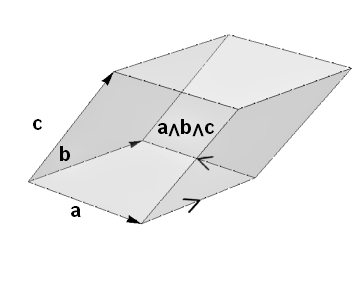
\includegraphics[width=.5\linewidth]{Fall_2017_Math_Research_Paper_Visuals/Trivector}
			\caption{$\mathbf{a} \wedge \mathbf{b} \wedge \mathbf{c}$}
			\label{trivector}
		\end{figure}
	
%%%%%%%%%%%%%%%%%%%%%%%%%%%%%%%%%%%%%%%%%%%%%%%%%%%%%%%%%%%%%%%%%%%%%%%%%%%%%%%%%%%%%%%%%%%%%%%%%%%%%%%%%%%%%%%%%%%%%%%%%%%%%%%%%%%%%%%%%%%%%%%%%%%%%%%%%%%%%%%%%%%%%%%%%%%%%%%%%%%%%%%%%%%%%%%%%%%%%%%%%%%%%%%%%%%%%%%%%%%%%%%%%%%%%%%%%%%%%%%%%%%%%%%%%%%%%%%%%%%%%%%%%%%%%%%%%%%%%%%%%%%%%%%%%%%%%%%%%%%%%%%%%%%%%%%%%%%%%%%%%%%%%%%%%%%%%%%%%%%%%%%%%%%%%%%%%%%%%%%%%%%%%%%%%%%%%%%%%%%%%%%%%%%%%%%%%%%%%%%%%%%%%%%%%%%%%%%%%%%%%%%%%%%%%%%%%%%%		
	\section{Implications} \label{implications}
		The cross product is taught usually during the latter part of the calculus sequence, at the same time students are taught about vectors, but the exterior product is derived in exterior algebra, a much higher level course than calculus. Students in calculus do not necessarily have the necessary prerequisites to fully understand what is happening with the exterior product, so instead of excluding it from their education, the cross product was created as an adaptation of the exterior product for three-dimensions so that students can still reap the benefits of the properties of these bi-vectors and tri-vectors without having to fully understand what is actually happening behind the scenes. Although creating this adaptation sacrifices the geometric intuition associated with creating tangent planes and finding volumes, it saves the students from being overwhelmed by having to deal with multi-vectors when they have yet to become fully comfortable with standard vectors. Regardless of the reasoning behind creating this adaptation of the exterior product, realizing what is actually happening when a cross product or a triple scalar product operation is performed provides a much clearer approach to visualizing why these seemingly random operations have such important attributes.

%%%%%%%%%%%%%%%%%%%%%%%%%%%%%%%%%%%%%%%%%%%%%%%%%%%%%%%%%%%%%%%%%%%%%%%%%%%%%%%%%%%%%%%%%%%%%%%%%%%%%%%%%%%%%%%%%%%%%%%%%%%%%%%%%%%%%%%%%%%%%%%%%%%%%%%%%%%%%%%%%%%%%%%%%%%%%%%%%%%%%%%%%%%%%%%%%%%%%%%%%%%%%%%%%%%%%%%%%%%%%%%%%%%%%%%%%%%%%%%%%%%%%%%%%%%%%%%%%%%%%%%%%%%%%%%%%%%%%%%%%%%%%%%%%%%%%%%%%%%%%%%%%%%%%%%%%%%%%%%%%%%%%%%%%%%%%%%%%%%%%%%%%%%%%%%%%%%%%%%%%%%%%%%%%%%%%%%%%%%%%%%%%%%%%%%%%%%%%%%%%%%%%%%%%%%%%%%%%%%%%%%%%%%%%%%%%%%%		
	\newpage
	\begin{thebibliography}{10}
		\begin{comment}
			\bib{BW}{article}{
			author = {Last, First},
			title = {Title},\usepackage{amsmath}
			date = {Date},
			journal = {Journal},
			volume = {Volume},
			number = {Number},
			pages = {start page\ndash end page},
			organization = {Organization},
			address = {Address}
			doi = {Number},
			url = {URL}
			}
		\end{comment}

		
		\bib{Gan13}{miscellaneous}{
			author = {Ganatra, S.},
			title = {Wedge Products and the Determinant},
			date = {Spring 2013},
			address = {Los Angeles},
			eprint = {http://www-bcf.usc.edu/~sheelgan/spring2013_math113/notes/wedge_products.pdf}
		}
		\bib{Hit}{miscellaneous}{
			author = {Hitchin, N.},
			title = {Exterior Algebra},
			address = {Oxford},
			eprint = {https://people.maths.ox.ac.uk/hitchin/hitchinnotes/Projective_geometry/Chapter_3_Exterior.pdf}
		}
		\bib*{WSC17}{conference}{
			title = {World Society for Computer Graphics Conference},
			address = {Plze\u{n}, Czech Republic},
			date = {2017}
		}
		\bib{Len17}{misc}{
			author = {Lengyel, E.},
			title = {A Bigger Mathematical Picture for Computer Graphics},
			xref = {WSC17}
		}
		\bib{Wed17}{article}{
			author = {Ganatra, Sheel},
			title = {Wedge Product and Their Use in Euclidean 3D Geometry},
			date = {December 2014},
			eprint = {https://lobishomen.wordpress.com/2014/12/24/wedge-product-and-their-use-in-euclidean-3d-geometry/}
		}
		
	\end{thebibliography}
\end{document}